\documentclass{article}
\usepackage[utf8]{inputenc}
\usepackage[margin=1in]{geometry}
\usepackage{graphicx}

\title{Math Clinic Status Update 2}
\author{Team 1: Komi Agbo, Dalton Burke, Nick Mako, James Vance}
\date{November 4th, 2019}

\begin{document}

\maketitle

\section{Since our last update...}
We have written some code for randomly generating data, creating the matching 
(and visualizing it) with the Hungarian Algorithm, setting up the star route, 
finding good transition candidates. Currently, there is a bug with the matching
(inter-zone matchings sometimes perform worse than zone restricted matchings on
the same data), and we need to refactor star route and transition candidate code
so that it uses the correct objects.

\begin{center}
	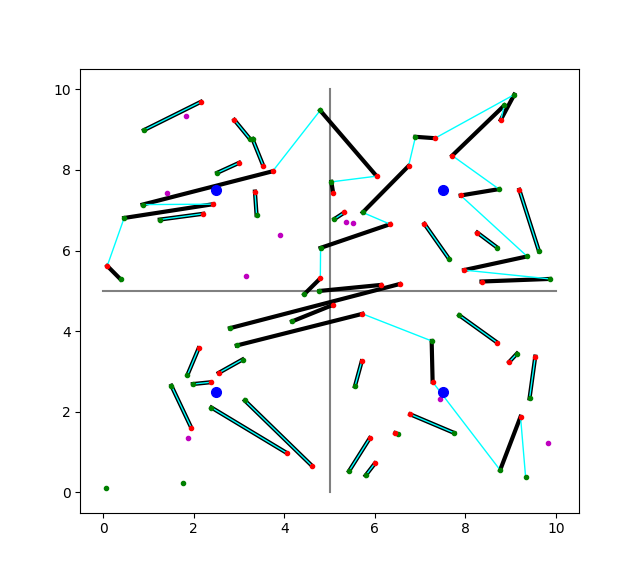
\includegraphics[scale=.75]{img/matching_demo.png}\\
	Matching visualization, blue points are landfills, green points are deliveries,
	red points are 	pickups. Cyan lines are the matching when deliveries and pickups
	can only be matched when they are in the same landfill zone, and black lines are 
	the matching when they are allowed to cross zones.
\end{center}

We also discovered that when allowing for DP pairs to straddle zones, they can end up
sending way too many drivers to a particular zone, where it will be inefficient to move 
them from later. The estimates for their weights seem to not be too far off from the 
matching with no inter-zone travel, it may be better to pick inefficient transitions 
from this case than to try to modify inter-zone to only have so many transitions.

\section{What's on our plate now...}
\begin{itemize}
  \item Work more on making good transitions
  \item Integrate data that the professor published
  \item Fix bugs
  \item Refactor star/transition code
\end{itemize}
\section{What's next...}
\begin{itemize}
  \item Satisfy other constraints for driver routes
  \item Satisfy inventory constraints for landfills
\end{itemize}

\end{document}

